\chapter{Исследовательский раздел}

\section{Постановка исследования}

Цель исследования --- выявление зависимости задержки аудио и видео, а также общей нагрузки на процессор от числа участников в конференции.

Исследование проведено на ноутбуке Intel i5-8365U 4.1GHz, 16GB оперативной памяти, под операционной системой Debian 12.

Количество участников варьируется от 2 до 7, время конференции --- 1 минута. Во время конфереции все участники транслировали одно и то же видео.

\section{Результаты}

Результаты представлены на графике \ref{img:latency}.

\begin{figure}[h!]
  \centering
  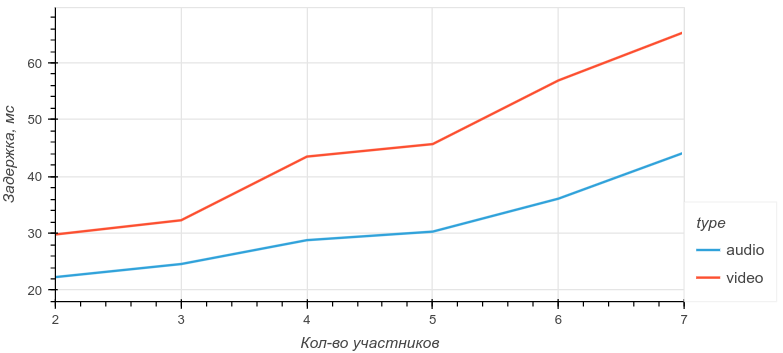
\includegraphics[width=\linewidth]{inc/img/latency.png}
  \caption{Зависимость средней задержки аудио и видео от числа участников конференции}
  \label{img:latency}
\end{figure}

На основе полученных результатов можно предположить, что увеличение задержки связанно с  увеличивающейся нагрузкой на процессор при увеличении количества участников.

% \section*{Выводы}
